\section{Results}

\begin{table}[h!]
\centering
\caption{Period 0. Limit 1800\,s. Means over ten runs. Status refers to scalar MLU~\eqref{eq:mlu}.}
\label{tab:t0}
\renewcommand{\arraystretch}{1.15}
\footnotesize
\setlength{\tabcolsep}{4.5pt}
\begin{tabular}{@{}lrrrrrrrl@{}}
\toprule
\textbf{Instance} & \textbf{$|V|$} & \textbf{$|A|$} & \textbf{$|D|$} &
\textbf{MLU} & \textbf{Time (s)} & \textbf{Gap} & \textbf{Nodes} & \textbf{Status} \\
\midrule
setA-01 & 20 & 80 & 40 & 0.9294 & 1.05 & 0 & 1 & MLU-opt. \\
setA-02 & 30 & 150 & 45 & 0.5486 & 2.79 & 0 & 1 & MLU-opt. \\
setA-03 & 50 & 250 & 20 & 0.9435 & 39.43 & 0 & 1 & MLU-opt. \\
setA-04 & 50 & 250 & 200 & 0.4591 & 1744.0 & $1.12\times 10^{-4}$ & 105.7 & Not cert. \\
setA-05 & 100 & 396 & 100 & 0.1155 & 0.03 & 0 & 0 & MLU-opt. \\
setA-06 & 100 & 500 & 500 & 0.0986 & 352.3 & 0 & 795 & MLU-opt. \\
setA-07 & 100 & 500 & 800 & 0.9080 & 0.03 & 0 & 0 & MLU-opt. \\
setA-08 & 150 & 654 & 200 & 0.3189 & 2.69 & 0 & 2.1 & MLU-opt. \\
setA-09 & 150 & 750 & 200 & 0.5054 & 0.04 & 0 & 1 & MLU-opt. \\
setA-10 & 150 & 966 & 1000 & 0.0761 & 1739.3 & 0.1020 & 272.6 & Not cert. \\
setA-11 & 200 & 1000 & 400 & 0.6555 & 1741.0 & 0.0646 & 1.3 & Not cert. \\
setA-12 & 200 & 898 & 400 & 0.6401 & 1299.3 & 0.0955 & 9.9 & Not cert. \\
setA-13 & 200 & 1000 & 2000 & 0.0389 & 1741.5 & $9.99\times 10^{-4}$ & 2690.6 & Not cert. \\
setA-14 & 250 & 1108 & 600 & 0.4240 & 1745.2 & $1.43\times 10^{-4}$ & 119.2 & Not cert. \\
setA-15 & 250 & 1250 & 600 & 0.8252 & 0.04 & 0 & 0 & MLU-opt. \\
setA-16 & 250 & 1452 & 4800 & 0.0393 & 1787.0 & 0.0172 & 12398.5 & Not cert. \\
setA-17 & 300 & 1270 & 2000 & 0.4242 & 0.05 & 0 & 0 & MLU-opt. \\
setA-18 & 300 & 1500 & 2000 & 0.6334 & 0.04 & 0 & 0 & MLU-opt. \\
setA-19 & 300 & 1998 & 6000 & 0.0483 & 1774.2 & 0.0296 & 8516.1 & Not cert. \\
setA-20 & 400 & 2000 & 6000 & 0.9913 & 0.09 & 0 & 0 & MLU-opt. \\
\bottomrule
\end{tabular}
\end{table}

On period~0, twelve of the twenty instances are MLU-optimal.
Several certificates arrive in well under a second, including setA-20 ($|V|=400$, $|D|=6000$),
where the column-generation bound meets the incumbent at the root.
The other eight instances consume essentially the full 1800\,s budget.
setA-04, setA-13 and setA-14 stop with a gap below $10^{-3}$; setA-10--12 remain between
6\% and 10\% above the bound.

\begin{table}[h!]
\centering
\caption{Periods 0 and 1 with budget. Limit 3600\,s. Status refers to scalar MLU~\eqref{eq:mlu}.}
\label{tab:full}
\renewcommand{\arraystretch}{1.15}
\footnotesize
\setlength{\tabcolsep}{4.5pt}
\begin{tabular}{@{}lrrrrrrrl@{}}
\toprule
\textbf{Instance} & \textbf{$|V|$} & \textbf{$|A|$} & \textbf{$|D|$} &
\textbf{MLU} & \textbf{Time (s)} & \textbf{Gap} & \textbf{Nodes} & \textbf{Status} \\
\midrule
setA-01 & 20 & 80 & 40 & 0.9294 & 14.61 & 0 & 1 & MLU-opt. \\
setA-02 & 30 & 150 & 45 & 0.9031 & 152.7 & 0 & 1 & MLU-opt. \\
setA-03\textsuperscript{a} & 50 & 250 & 20 & 0.9437 & 1430.5 & 0.0030 & 33.1 & Not cert. \\
setA-04 & 50 & 250 & 200 & 0.5812 & 3592.7 & $1.61\times 10^{-4}$ & 1503.4 & Not cert. \\
setA-05 & 100 & 396 & 100 & 0.2050 & 0.32 & 0 & 1 & MLU-opt. \\
setA-06 & 100 & 500 & 500 & 0.0986 & 168.0 & 0 & 540.8 & MLU-opt. \\
setA-07 & 100 & 500 & 800 & 0.9080 & 42.32 & 0 & 229.6 & MLU-opt. \\
setA-08 & 150 & 654 & 200 & 0.3189 & 1.26 & 0 & 3 & MLU-opt. \\
setA-09 & 150 & 750 & 200 & 0.8497 & 2.60 & 0 & 2 & MLU-opt. \\
setA-10 & 150 & 966 & 1000 & 0.0733 & 3594.1 & 0.0678 & 4947 & Not cert. \\
setA-11 & 200 & 1000 & 400 & 0.7858 & 2.92 & 0 & 2 & MLU-opt. \\
setA-12 & 200 & 898 & 400 & 0.8799 & 1.82 & 0 & 2 & MLU-opt. \\
setA-13 & 200 & 1000 & 2000 & 0.0420 & 3591.1 & 0.0288 & 7846.2 & Not cert. \\
setA-14 & 250 & 1108 & 600 & 0.5176 & 3608.9 & 0.0197 & 17922.4 & Not cert. \\
setA-15 & 250 & 1250 & 600 & 0.8987 & 5.61 & 0 & 1 & MLU-opt. \\
setA-16 & 250 & 1452 & 4800 & 0.1369 & 3594.2 & 0.6682 & 32238.2 & Not cert. \\
setA-17 & 300 & 1270 & 2000 & 0.4242 & 50.51 & 0 & 1 & MLU-opt. \\
setA-18 & 300 & 1500 & 2000 & 1.0000 & 32.79 & 0 & 0 & MLU-opt. \\
setA-19 & 300 & 1998 & 6000 & 0.1096 & 3542.7 & 0.5586 & 15254 & Not cert. \\
setA-20 & 400 & 2000 & 6000 & 0.9913 & 401.9 & 0 & 2 & MLU-opt. \\
\bottomrule
\end{tabular}\\[0.3em]
{\footnotesize\textsuperscript{a}\,Eight runs are MLU-optimal at $0.9435$; two stop at $0.9444$.}
\end{table}

\begin{figure}[h!]
\centering
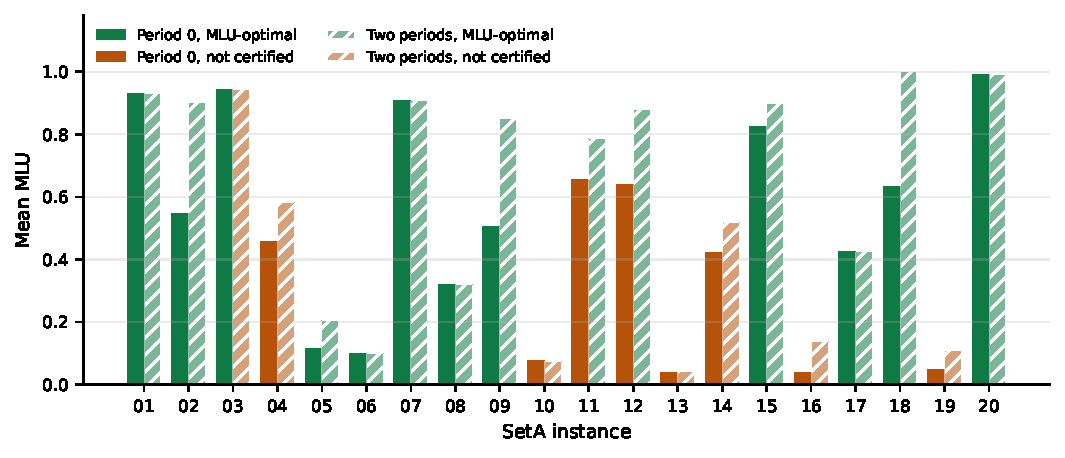
\includegraphics[width=\linewidth]{mlu_compare.pdf}
\caption{Mean MLU on period~0 (solid bars) and on both periods (hatched).
Green: all ten runs certified for~\eqref{eq:mlu}; amber: not certified.}
\label{fig:mlu}
\end{figure}

Thirteen two-period instances are MLU-optimal.
Adding period~1 does not change the reported MLU of setA-01, 06, 07, 08, 17 and 20: a feasible
routing meets the budget without raising the peak load (for the certified rows among them,
this equality is proven).
Elsewhere the second period raises the peak: setA-02 from $0.5486$ to $0.9031$, setA-05 from
$0.1155$ to $0.2050$, setA-09 from $0.5054$ to $0.8497$, and setA-18 from $0.6334$ to $1$.
setA-11 and setA-12 are not certified on period~0, yet their higher two-period values
$0.7858$ and $0.8799$ are certified.
setA-03 is mixed: eight runs prove $0.9435$ and two stop at $0.9444$.
